\documentclass[onecolumn, draftclsnofoot,10pt, compsoc]{article}
\usepackage{graphicx}
\usepackage{url}
\usepackage{lscape}
\usepackage{setspace}
\usepackage{parskip}
\usepackage{geometry}
\usepackage{listings}
\usepackage{subfiles}
\usepackage{pdfpages}
\usepackage{graphicx}
\geometry{textheight=9.5in, textwidth=7in}

% 1. Fill in these details
\def \CapstoneTeamName{AgBizClimate}
\def \CapstoneTeamNumber{26}
\def \GroupMemberOne{Thomas Noelcke}
\def \GroupMemberTwo{Shane Barrantes}
\def \GroupMemberThree{Shengpei Yuan}
\def \CapstoneProjectName{ Linking Seasonal Weather Data to AgBizClimate\texttrademark}
\def \CapstoneSponsorCompany{ Oregon State University}
\def \CapstoneSponsorPerson{ Clark Seavert}

% 2. Uncomment the appropriate line below so that the document type works
\def \DocType{		%Software Requirements Document
				%Requirements Document
				%Technology Review
				%Design Document
				Final Document
				}

\newcommand{\NameSigPair}[1]{\par
\makebox[2.75in][r]{#1} \hfil 	\makebox[3.25in]{\makebox[2.25in]{\hrulefill} \hfill		\makebox[.75in]{\hrulefill}}
\par\vspace{-12pt} \textit{\tiny\noindent
\makebox[2.75in]{} \hfil		\makebox[3.25in]{\makebox[2.25in][r]{Signature} \hfill	\makebox[.75in][r]{Date}}}}
% 3. If the document is not to be signed, uncomment the RENEWcommand below
%\renewcommand{\NameSigPair}[1]{#1}

%%%%%%%%%%%%%%%%%%%%%%%%%%%%%%%%%%%%%%%
\begin{document}
\begin{titlepage}
    \pagenumbering{gobble}
    \begin{singlespace}
        \hfill
        % 4. If you have a logo, use this includegraphics command to put it on the coversheet.
        %\includegraphics[height=4cm]{CompanyLogo}
        \par\vspace{.2in}
        \centering
        \scshape{
            \huge CS Capstone \DocType \par
            {\large\today}\par
            \vspace{.5in}
            \textbf{\Huge\CapstoneProjectName}\par
            \vfill
            {\large Prepared for}\par
            \Huge \CapstoneSponsorCompany\par
            \vspace{5pt}
            {\Large\NameSigPair{\CapstoneSponsorPerson}\par}
            {\large Prepared by }\par
            Group\CapstoneTeamNumber\par
            % 5. comment out the line below this one if you do not wish to name your team
            %\CapstoneTeamName\par
            \vspace{5pt}
            {\Large
                \NameSigPair{\GroupMemberOne}\par
                \NameSigPair{\GroupMemberTwo}\par
                \NameSigPair{\GroupMemberThree}\par
            }
            \vspace{20pt}
        }
        \begin{abstract}
			The purpose of this document is to provide documentation regarding the \textit{AgBizClimate} project. We will start off the document by giving a general overview of the \textit{AgBizClimate Project}. This will inclue information about the goals of the project, and information about the project stakeholders. Next we have our requirements document. In this section we will also discuss how our requirements have changed over the last several terms. Next we will be discussing the design document. In this section we will first display our original design document. We will then discuss how our design has changed over the term. After the design document we will display the tech review. Next, we will also display the project poster. Finally we will provide some project documentation regarding how project setup, running the project, how the project works and guids for any API's we are using. After this we will discuss any technical resources for learning more about the technologies that our project uses. Finally, We will end this document with our conclusions and reflections section. This section will involve reflecting on this project and discussing what went well and what didn't go well.\\
        \end{abstract}
    \end{singlespace}
\end{titlepage}
\newpage
\pagenumbering{arabic}
\tableofcontents
% 7. uncomment this (if applicable). Consider adding a page break.
%\listoffigures
\newpage
%\listoftables
\clearpage

% 8. now you write!
% Will need to review this section to make sure its accurate and that it covers all the bullet points in the
% requirements for this section.
\section{Introduction}

		\subsection{The Team}
		    \paragraph{Thomas Noelcke} Through out this project Thomas played the role of team lead as well as front end developer and atmospheric science technical expert.\\

		    \paragraph{Shane Barantes} This project depended on Shanes skills in devops and environment setup as well as back end web programming.\\

		    \paragraph{Shengpei Yuan} Shempei was our python expert as well as our QA testing expert.\\

		\subsection{Project Sponsors}
		    This project was sponsored by Clark Seavert from OSU the applied economics department at Oregon State University. Professor Seavert specializes in Enterprise budgets, capital investments, and crop and livestock leasing.\\

        \subsection{Client Involvement}
            Clark Seavert was largely hands off during this project. However, that's not to say he didn't play a role. Clark was very helpful we reviewing documents and presentations. Clark also provided timely feed back on any change requests to the project.\\

            It is also important to note that though our project sponsor was not directly involved in the development of the short term climate tool his project manage Sean Hammond was a great resource through out the project. Through out the project we worked with Sean to work through technical problems and road blocks. Through out the term we met with Sean on a weekly basis to discuss progress on the project along with any major blockers. During these meetings Sean provided guidance on any problems we may have run into.\\

		\subsection{Definitions, Acronyms and Abbreviations}
			REST - Representation State Transfer, This is a type of architecture that manages preforms operations on the state of the program. This is especially popular in web development.\\
			API- Application Programming Interface. This is a piece of software that allows a connection to another piece of software providing some sort of service.\\
			Thredds Data Server - This is a web server that provides meta-data and data access for scientific data sets using OPeNDAP along with some other remote data access protocols.\\
			OPeNDAP - Open-source Project for a Network Data Access Protocol. This is the protocol we will be using to retrieve the data sets from the Thredds data server.\\
			NMME - North American Multi-Model Ensemble. This is a data set that brings together a variety of different weather models into one data set.\\
			Climate Scenario - This is a theoretical calculation of yields, inputs and of the overall budget for one situation based on the climate data.\\
			NETCDF - This is a file storage format for large scientific data sets especially good for any data that is referenced on a grid and related to is geo-location.\\
			SQL Database - This is a relational database that makes storing and accessing data easy.\\
			Container - A virtualized operating system that is used to host and deploy web development projects. This allows projects to be easily portable between different operating systems and platforms.\\
			Mount Bind - This is the practice of mounting a directory from the native os to the container such that if either the container or the native operating system. This allows changes in the files to be reflected in both the container and the native operating system.\\


			\renewcommand\refname{\vskip -1cm}
		\subsection{References}

		\nocite{*}
    \bibliographystyle{IEEEtran}
    \bibliography{IEEEabrv,References}


		\subsection{Overview}
			Seasonal climate is one of the essential factors that affects harvest, returns of crops and farming investment programs of enterprises and organizations. As a sub-project of AgBizLogic, AgBizClimate is dedicated to deliver essential information about climate change to farmers, and help professionals to develop management pathways that best fit their operations under a changing climate. This project aims to link the crucial seasonal climate data from the Northwest Climate Toolbox database to AgBizLogic so that it can provide specific analysis and illustrations through powerful graphics. AgBizClimate is designed to enable farmers and agriculture enterprises to decide appropriate farming investment projects for their crops and products.\\

            Currently AgBizClimate has a long-term climate tool but no such tool exists for short term climate data. We will implement a tool to extract short-term climate data from the Northwest Climate Toolbox database, display it to the user and allow the user to adjust crop yields, inputs and costs. Moreover, a landing tool will be developed to allow users to switch between short term seasonal tool and long-term climate data tool.\\

            Seasonal weather data is important for farmers and land managers as climate has great impact on crops. For instance, the precipitation on different days across the life cycles of crops may have different impacts on the harvest. Land managers and farmers used to rely on past experiences of climate to make decisions for specific farming operations to reduce the negative impacts and make use of favorable climate conditions. However, these individual experiences of weather data are often limited and inaccurate. Professional tools like software systems could be adopted to build models for decision making based on available seasonal climate data.\\

    \subsection{Project Scope}
		This project is a part of a much larger AgBiz Logic\texttrademark program. However, the purpose of this project is to add a short term climate tool to the \textit{AgBizClimate} module. This limits the scope of the project to the \textit{AgBizClimate} Module. Additionally, we will only be adding the short term climate data tool as the long term climate data tool already exists.\\



	\subsection {Product Functions}
			\textit{AgBizClimate} is a web based decision tool that will allow users to gain specific insight on how localized climate data for the next seven months will affect their crop and livestock yields or quality of products sold and production inputs. The \textit{AgBizClimate} tool will allow users to input their location (state, county) and a budget for the specific crop or livestock enterprise. \textit{AgBizClimate} will select climate data for the next seven months for that location and provide graphical data showing temperature and precipitation. Users will then be able to change yields or quality of product sold by a percentage they think these factors will affect and modify production inputs. Finally the tool will calculate the net returns.\\

	\subsection{User Characteristics}
		\textit{AgBizClimate} users can be split into two subgroups, agricultural producers and climate researchers. The first subgroup, agricultural users who use this product tend to be between fifty and sixty years old of mixed gender. Their educational background ranges from high school to the completion of college. The primary language this group uses is English, but there are some Spanish users as well. Most of the users in this group tend to have novice computational skills. The primary domain for these users is agricultural and business management. Most agricultural producers who use this product are motivated by the potential profit that the decision tool \textit{AgBizClimate} could potentially offer. The second subgroup, climate researchers range from ages twenty to forty and are of mixed gender. The educational background for most climate researchers  exceed the postgraduate level with their primary language being English. These users generally have advanced computational skills and are motivated by the easily accessible climate and weather data.\\

	\subsection{Constraints}
		There are several key constraints that this product has to work within. Firstly, We are limited by the availability and completeness of the data from the NMME data set. The NMME Data set does not have data for every point on in the country. Secondly, we must use the Threadds server hosted by University of Idaho to get the data in the NetCDF format. The tooling provides a variety of access methods however, the only method that currently works is downloading the whole file. Fourthly, we don’t have access to any of the hardware that \textit{AgBizClimate} is exists on as it is being managed by a third party. This will prevent us from improving the hardware or cause roadblocks if their servers are having issues. Lastly, we are limited to using the languages Python and JavaScript since we are integrating our product into an already existing project.\\

	\subsection {Assumptions and Dependencies}
		We are assuming that the NMME Thredds data base will allow us to pull location based temperature and precipitation data. This data will come in the form of a NetCDF files which we will then read and format a JSON response. Due to the fact that we are writing an addition to an existing project we do not need to interact with the user budgets as these have already been defined. This fact extends to the calculations portion of the \textit{AgBizClimate} product. Our team will simply be accessing data via the NMME threadds database, will then format the data, store the data, and hand the data over to the front end or some other sort of client.\\


\section{Requirements Document}
    \subsection{Original Document}
        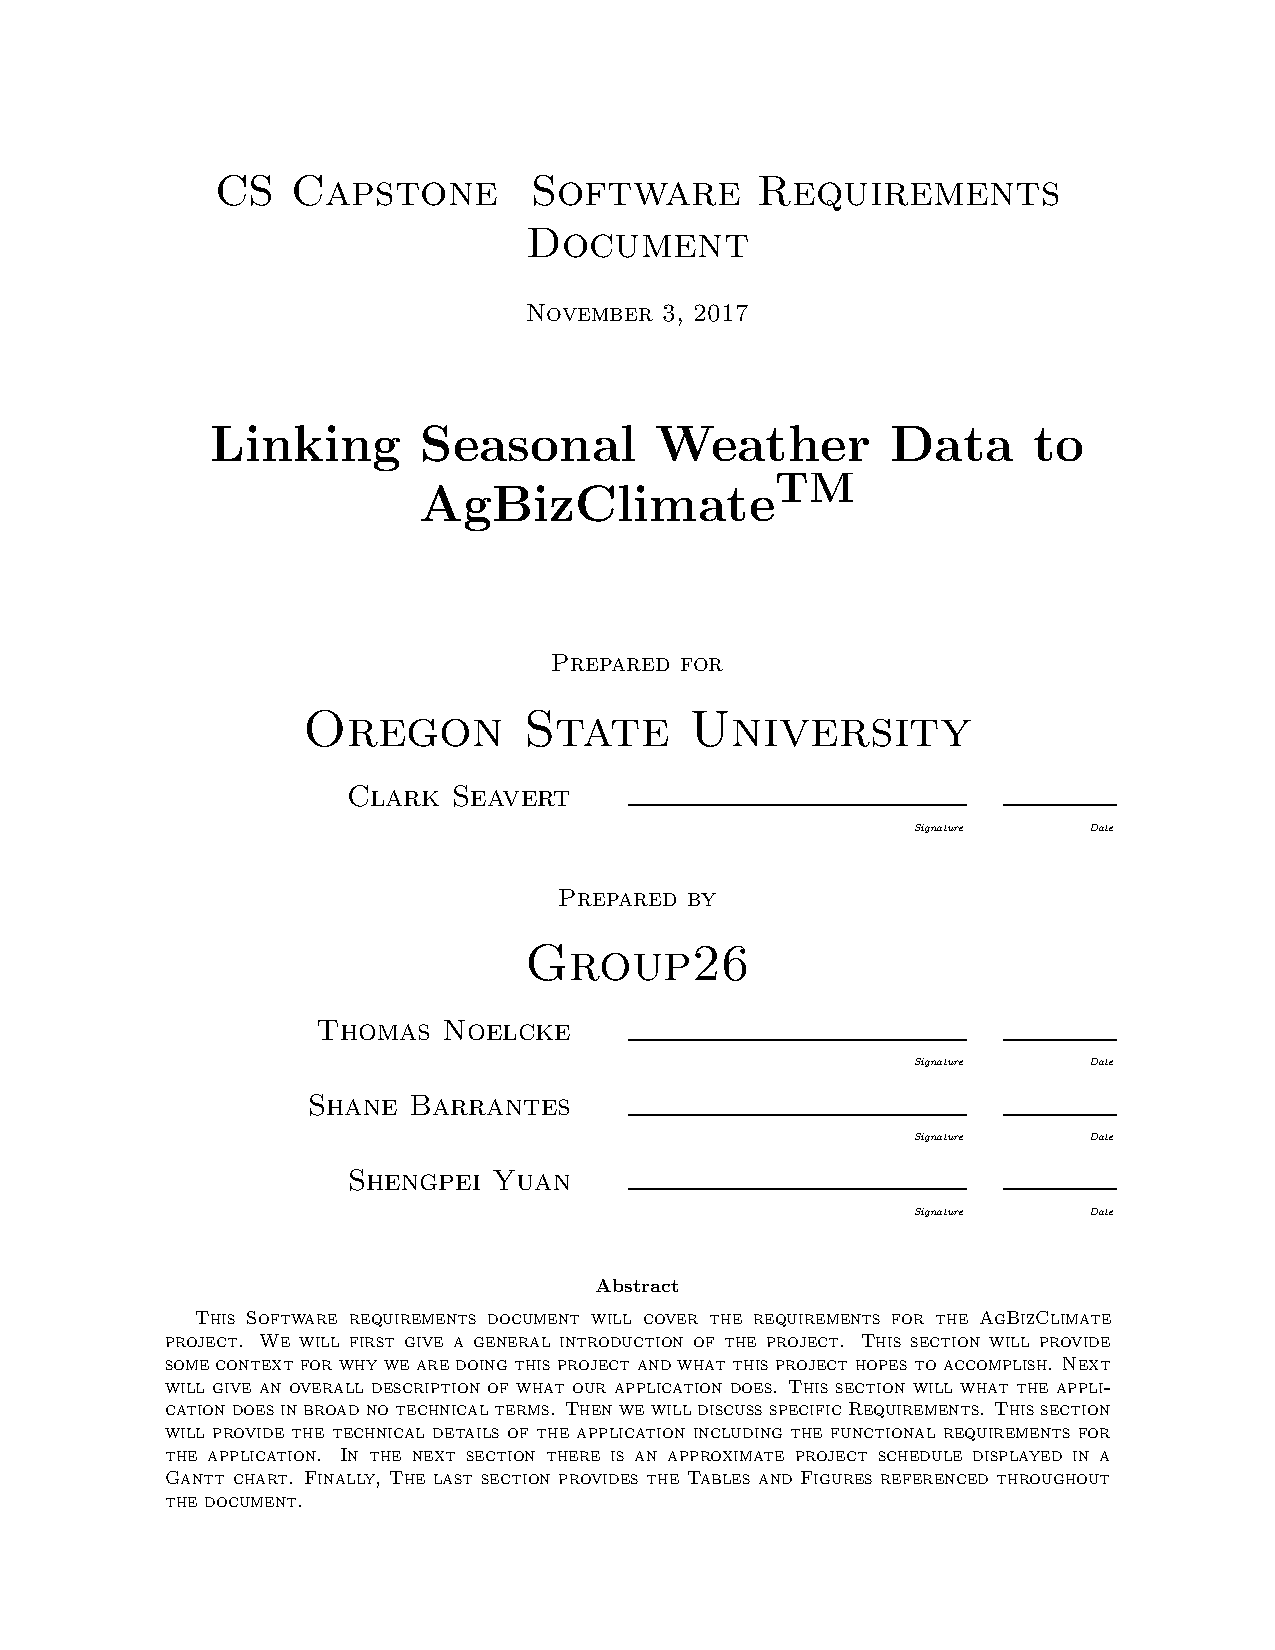
\includepdf[pages={1-16}]{./Original-Docs/Requirements-Document-Original/AgBizClimateSRS.pdf}

    \subsection{Changes}

        \subsubsection{Introduction}
	    Through out this process some things mentioned above the introduction has changed to reflect the changes to the application. Specifically, We are no longer using NWCTB as we had originally assumed. Instead we are using a Threadds server hosted by the university of Idaho. As such we would change the references to the NWCTB to NMME Threadds database.\\

	    \subsubsection{Overall description}
	    Several things changed over the term in the overall descriptions section, constraints, and Assumptions and Dependencies. The constraints changed because we were originally thinking we were going to be required to use the NWCTB API to get the data. Instead of the NWCTB were actually constrained by the downscale NMME Threadds database hosted at University of Idaho. The assumptions and dependencies for similar reasons. We were originally assuming that we were going to need to use the NWCTB to get the data. However, because we ended using the Threadds database this introduced a slew of new dependencies including, netcdf4, the OPeNDAP protocol and HDF5.\\

	    \subsubsection{User Interface Changes}
	    Through out the process of building this application we found that there were a variety of changes were made to the UI design we originally proposed. Below we will discuss the changes we made to the UI. We will break down these changes by section as that's how it was done in the design document. Each section represents a page.\\

	        \paragraph{Landing page}
	         Originally we though we were going to use the climate manager page to branch between the different climate scenario types. We were going to do this using a button that would create a new short term climate scenario. We ended up choosing to branch a bit later in the process as it made our application simpler. As such the climate manager now only contains one button to create a new climate scenario. The climate manager also allows you to review old scenarios and to delete old scenarios. This was not functionality included in the original document.\\

	        \paragraph{New Climate Scenario Page}
	        The New Climate Scenario page design was more or less unchanged however we did not adequately describe the page in our initial requirements document. We never specified that the user would be able to add up to five budgets using this page.\\

	        \paragraph{Region Select Page}
	        Originally, the region select page was just going to be to select the region. However, early on in development we realized that if we had our user select the region and forecast scope on this page that it would simplify our work flow. So instead of just selecting state and county the user now selects climate forecast type, state and county. We also did not mention that the user will not be allow to continue with out entering all three of these items.\\

	        \paragraph{Charts Page}
	        In our initial draft of our requirements document we had planed to use a drop down menu to allow the user to select different plots that they might want to look at. We decided that it would be better to use tabs for the same functionality. So now the user may switch between different charts using tabs rather than using a drop down menu.\\

	        \paragraph{Climate Summary Page}
	        We added a new page to the User Interface description. In our original requirements document we did not know we would have a summary page, however the client already had a summary page implemented that we were able to plug the data we created in the short term tool. This page allows the user to see a summary and visual representation of what they did during their short term scenario.\\

        \subsubsection{Interfaces}
        Given that the source of our data changed we also made some changes to the hardware and software interfaces. The big change to the hardware interface is that we are now using a Threadds server located at the university of Idaho. Previously we were assuming we would be able to use the NWCTB to get the data.\\

        We also made some changes the software interface. Given that the source of our data changed several times through out the term we are no longer using the NWCTB to get our data. In fact we are now downloading the data monthly and placing in on the dev server. We are then passing the file to the container our application is run in via a mount bind. As such the software interfaces for our application changed drastically over the term. We now have to include the dev server as part of our software interface. It is also important to note that we are interfacing with the Threadds server at University of Idaho.\\

        \subsubsection{Functional Requirements changes}
            In this section we will discuss how the functional requirements have changed through out the course of the project. We will only discuss the requirements that have changed and will not discuss requirements that have not changed.\\

		    \paragraph{Functional Requirement 1.3: The data source}
		    As mentioned previously the source of the data changed from the NWCTB to the threads server hosted at University of Idaho. Additionally, the way our application uses this data changed through out the project. We were initially planning getting each data point as needed. However, we ended up storing the whole data file on the dev server.\\

		    \paragraph{Functional Requirement 1.4: Getting the Data}
		    In our original draft of the document we hadn't had a chance to look at the data yet and did not know that the data would be somewhat sparsely populated. So as the project moved along we realized that it would be possible to request a point and get NAN as a result even though it was in the middle of the data set. As such we were required to do some searching if the initial result was NAN. We eventually settled on searching with in a 20 mile radius as it was unlikely that there was not data with a 20 mile radius. We also realized that 20 miles was an acceptable margin for error.\\

		    \paragraph{Functional Requirement 1.5: Calculating Historical Data}
		    In our original document this requirement was actually sending a request for the data from the server. We swapped this requirement for calculating historic data because our client wanted to be able to see the projection vs the historical data and we are no longer making requests for the data as it is available locally.\\

		    \paragraph{Functional Requirement 1.6: Formatting the Data}
		    In our original document we were under the assumption that we would be sending a request for the data and processing the result. So this requirement changed from processing the data returned by our call to an API to formatting the data into a usable json object.\\

\section{Design Document}
    \subsection{Original Document}
        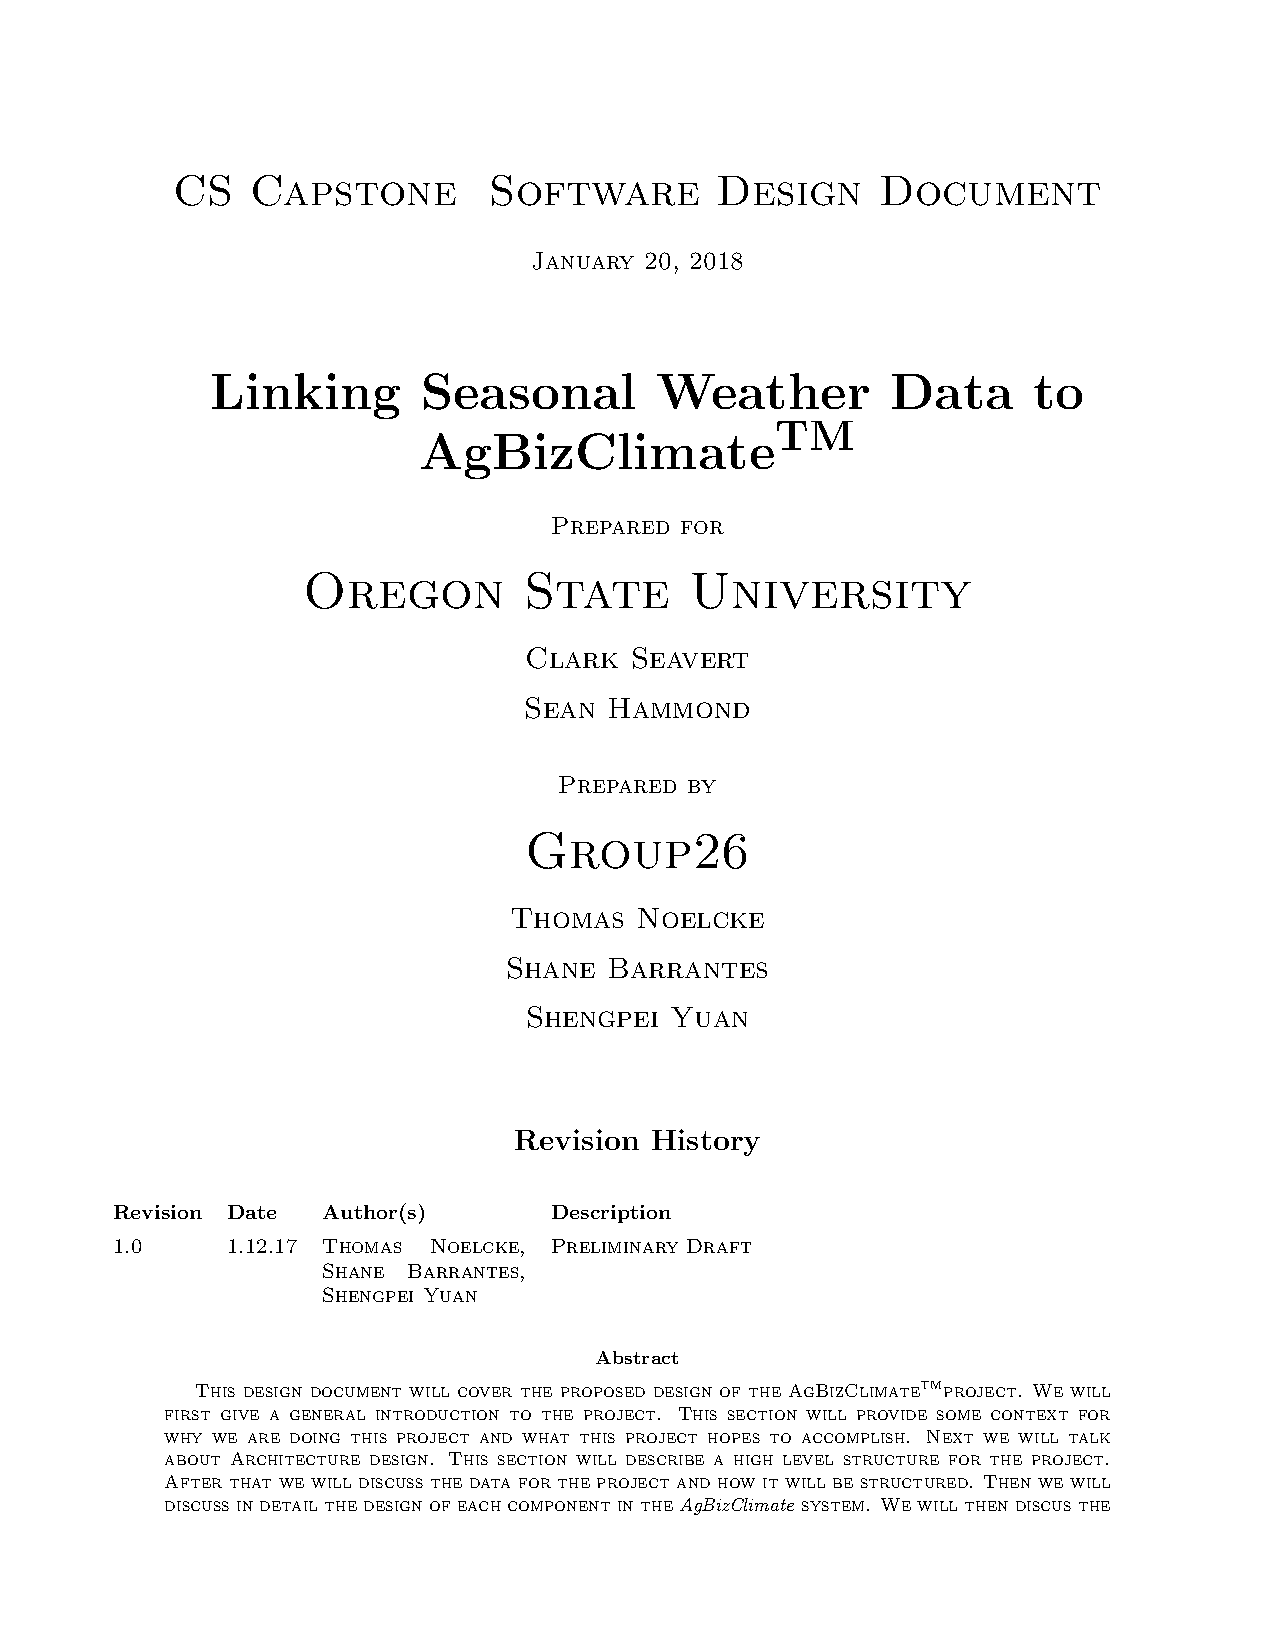
\includepdf[pages={1-33}]{./Original-Docs/DesignDoc/AgBizClimateDesignDoc.pdf}
    \subsection{Changes}

\section{Tech Review}
	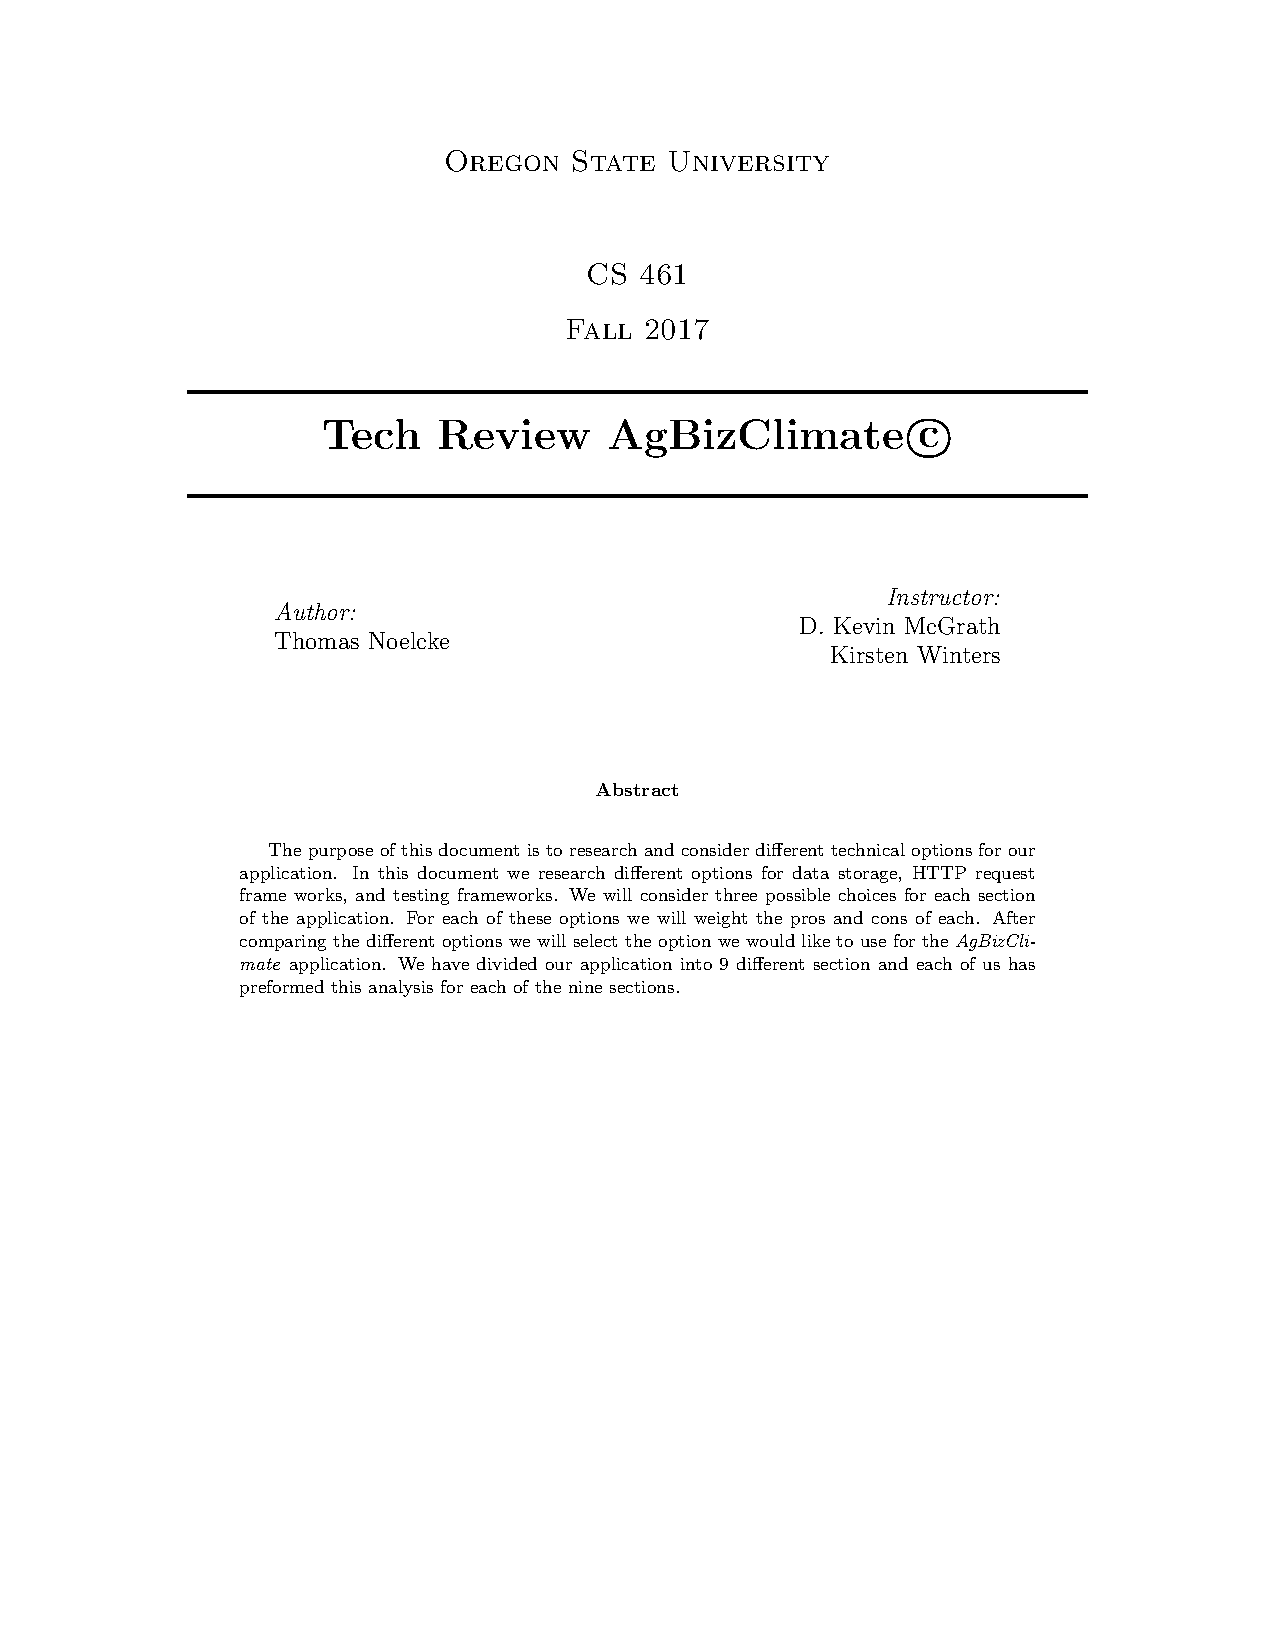
\includepdf[pages={1-23}]{./Original-Docs/Tech-Review/TechReviewCombined.pdf}

\section{Weekly Blog Posts}
    \subsection{Shane Barrantes}
        In This section I've imported the notes from my weekly OneNote updates. I will be denoting the term and week with the following format [Term Number].[Week].

        \subsubsection{Week 1.1}

		    \paragraph{Plans} \hfill \break

		    \paragraph{Problems} \hfill \break

		    \paragraph{Progress} \hfill \break

		    \paragraph{Summary} \hfill \break
		         I signed up for project preferences and reached out to multiple project managers, none responded back. \\

		\subsubsection{Week 1.2}

		    \paragraph{Plans} \hfill \break

		    \paragraph{Problems} \hfill \break

		    \paragraph{Progress} \hfill \break

		    \paragraph{Summary} \hfill \break
		        I was assigned to the agbiz project. I met with my group and we emailed the client to setup a meeting for Tuesday of next week.
		    \\

		\subsubsection{Week 1.3}

		    \paragraph{Plans} \hfill \break

		    \paragraph{Problems} \hfill \break

		    \paragraph{Progress} \hfill \break

		    \paragraph{Summary} \hfill \break
		    	\begin{itemize}
		        \item Met with client to get overview of project.
                \item Met with TA to better understand his role in project.
                \item Met with Senior tech of project to discuss the \item specifications of the project.
                \end{itemize}

		\subsubsection{Week 1.4}
			\paragraph{Plans} \hfill \break

		    \paragraph{Problems} \hfill \break

		    \paragraph{Progress} \hfill \break

		    \paragraph{Summary}
		    	\begin{itemize}
		            \item Met with group to make the final draft of the problem statement.
                    \item Signed a newly sprung NDA, will turn in early next week...
                    \item  Met with the TA.
                \end{itemize}


		\subsubsection{Week 1.5}

		    \paragraph{Plans} \hfill \break

		    \paragraph{Problems} \hfill \break

		    \paragraph{Progress} \hfill \break

		    \paragraph{Summary} \hfill \break
		    	\begin{itemize}
		            \item Turned in Problem statement.
                    \item Met with Client to discuss requirements document.
                    \item Met with the TA.\\
                \end{itemize}


		\subsubsection{Week 1.6}

		    \paragraph{Plans} \hfill \break

		    \paragraph{Problems} \hfill \break

		    \paragraph{Progress} \hfill \break

		    \paragraph{Summary} \hfill \
		        \begin{itemize}
		            \item Met with client to discuss the requirements \item document again.
                    \item Turned in rough draft of the requirements document.
                    \item Met with the TA. \\
                \end{itemize}


		\subsubsection{Week 1.8}

			\paragraph{Plans} \hfill \break

		    \paragraph{Problems} \hfill \break

		    \paragraph{Progress} \hfill \break

		    \paragraph{Summary}
		    \begin{itemize}
		    \item Turned in Rough draft of the technical review.
            \item Met with TA.
            \end{itemize}


		\subsubsection{Week 1.9}

			\paragraph{Plans} \hfill \break

		    \paragraph{Problems} \hfill \break

		    \paragraph{Progress} \hfill \break

		    \paragraph{Summary} \hfill \break
		    \begin{itemize}
                \item Meeting with TA cancelled.
                \item Worked on design document. \\
		     \end{itemize}
		\subsubsection{Week 1.10}

		    \paragraph{Plans} \hfill \break

		    \paragraph{Problems} \hfill \break

		    \paragraph{Progress} \hfill \break

		    \paragraph{Summary} \hfill \break
		        \begin{itemize}
                    \item Didn't meet with TA, got cancelled.
                    \item Finished/turned in design document.
                    \item Made progress report
                \end{itemize}

		  \subsubsection{Week 2.1}
			\paragraph{Plans} \hfill \break


			\paragraph{Progress} \hfill \break

			\paragraph{Problems} \hfill \break


			\paragraph{Summary} \hfill \break
			    \begin{itemize}
                    \item Met with the client
                    \item Got repo permissions
                    \item Set tasks
                \end{itemize}

		\subsubsection{Week 2.2}
			\paragraph{Plans}

			\paragraph{Progress} \hfill \break

			\paragraph{Problems} \hfill \break

			\paragraph{Summary}\hfill \break
			    \begin{itemize}
                    \item Met with the client
                    \item Defined API access
                \end{itemize}

		\subsubsection{Week 2.3}
			\paragraph{Plans} \hfill \break

			\paragraph{Progress} \hfill \break

			\paragraph{Problems} \hfill \break

			\paragraph{Summary} \hfill \break
				\begin{itemize}
                    \item Worked on concept script
                    \item Installed NetCDF and associated packages.
                \end{itemize}


		\subsubsection{week 2.4}
			\paragraph{Plans} \hfill \break

			\paragraph{Progress} \hfill \break

			\paragraph{Problems} \hfill \break

			\paragraph{Summary} \hfill \break
				\begin{itemize}
                    \item Met with the client
                    \item Defined API access
                \end{itemize}

		\subsubsection{week 2.5}
			\paragraph{Plans} \hfill \break

			\paragraph{Progress} \hfill \break

			\paragraph{Problems} \hfill \break

			\paragraph{Summary} \hfill \break
				\begin{itemize}
                    \item Met with the client
                    \item Worked on building NetCDF pipeline from source and all associated packages
                \end{itemize}

		%will fill out this section later this week.
		\subsubsection{week 2.6}
			\paragraph{Plans} \hfill \break

			\paragraph{Progress} \hfill \break

			\paragraph{Problems} \hfill \break

			\paragraph{Summary} \hfill \break
				\begin{itemize}
                    \item Finished development of the primary charts page
                    \item Completed the midterm progress report
                \end{itemize}

		\subsubsection{week 2.7}
			\paragraph{Plans} \hfill \break
		    \paragraph{Progress} \hfill \break
			\paragraph{Problems} \hfill \break
			\paragraph{Summary} \hfill \break
				\begin{itemize}
                    \item Showed client the alpha in meeting
                    \item Found a solution to bypass NetCDF to get climate data via URL
                \end{itemize}

		\subsubsection{week 2.8}
			\paragraph{Plans} \hfill \break

			\paragraph{Progress} \hfill \break

			\paragraph{Problems} \hfill \break

			\paragraph{Summary} \hfill \break
			    Completed the concept script which allowed us to get climate data while bypassing NetCDF.

		\subsubsection{week 2.9}
			\paragraph{Plans} \hfill \break

			\paragraph{Progress} \hfill \break

			\paragraph{Problems} \hfill \break

			\paragraph{Summary} \hfill \break
                Created API endpoint for the climate data and charts to pull from.

		\subsubsection{week 2.10}
			\paragraph{Plans} \hfill \break

			\paragraph{Progress} \hfill \break

			\paragraph{Problems} \hfill \break

			\paragraph{Summary} \hfill \break
			    Integrated the climate data API into the beta and showed it to the client.

		\subsubsection{Week 3.1}
		    \paragraph{Plans} \hfill \break

		    \paragraph{Progress} \hfill \break

		    \paragraph{Problems} \hfill \break

		    \paragraph{Summary} \hfill \break
				\begin{itemize}
                    \item Weren't able to get in contact with TA
                    \item Talked with team about plans for the term
                \end{itemize}

        \subsubsection{Week 3.2}
		    \paragraph{Plans} \hfill \break

		    \paragraph{Progress} \hfill \break

		    \paragraph{Problems} \hfill \break

		    \paragraph{Summary} \hfill \break
		            Found out that the API solution we spent months on doesn't actually work.


		\subsubsection{Week 3.3}
		    \paragraph{Plans} \hfill \break

		    \paragraph{Progress} \hfill \break

		    \paragraph{Problems} \hfill \break

		    \paragraph{Summary} \hfill \break
		        Tried R and MatLab NetCDF solutions for our API, however neither worked for this project.

		\subsubsection{Week 3.4}
		    \paragraph{Plans} \hfill \break

		    \paragraph{Progress} \hfill \break

		    \paragraph{Problems} \hfill \break

		    \paragraph{Summary} \hfill \break
		        Came up with a data mount solution for the climate API.

		\subsubsection{Week 3.5}
		    \paragraph{Plans} \hfill \break

		    \paragraph{Progress} \hfill \break

		    \paragraph{Problems} \hfill \break

		    \paragraph{Summary} \hfill \break
		        Created our midterm progress report.

		\subsubsection{Week 3.6}
		    \paragraph{Plans} \hfill \break

		    \paragraph{Progress} \hfill \break

		    \paragraph{Problems} \hfill \break

		    \paragraph{Summary} \hfill \break
		        Started creating back-end unit tests.

		\subsubsection{Week 3.7}
		    \paragraph{Plans} \hfill \break

		    \paragraph{Progress} \hfill \break

		    \paragraph{Problems} \hfill \break

		    \paragraph{Summary} \hfill \break
		    	\begin{itemize}
                    \item Finished creating the back-end unit tests
                    \item Attended Expo
                \end{itemize}

		\subsubsection{Week 3.8}
		    \paragraph{Plans} \hfill \break
		    \paragraph{Progress} \hfill \break
		    \paragraph{Problems} \hfill \break
		    \paragraph{Summary} \hfill \break
		        Finished final client recommended changes and re-based to master.

		\subsubsection{Week 3.9}
		    \paragraph{Plans} \hfill \break
		    \paragraph{Progress} \hfill \break
		    \paragraph{Problems} \hfill \break
		    \paragraph{Summary} \hfill \break
		        Recorded the Final Presentation.

		\subsubsection{Week 3.10}
		    \paragraph{Plans} \hfill \break

		    \paragraph{Progress} \hfill \break

		    \paragraph{Problems} \hfill \break

		    \paragraph{Summary} \hfill \break
		    	\begin{itemize}
                    \item Finished Final Document
                    \item Finished Final Report
                \end{itemize}


    \subsection{Thomas Noelcke}

        \subsubsection {Week 1.1}
        In this week our group had not yet been formed. As such there is no report for this week.
    \subsubsection{Week 1.1}

		    \paragraph{Plans} \hfill \break

		    \begin{itemize}
		        \item Set Up First Group Meeting
		        \item Meet With Client
		        \item Work On Problem Statement
		    \end{itemize}

		    \paragraph{Problems} \hfill \break

		    \begin{itemize}
		        \item Group Communication
		    \end{itemize}

		    \paragraph{Progress} \hfill \break
		    \begin{itemize}
		        \item Started Slack Channel with group 10/4
		        \item Contacted Client 10/4
		        \item met with group 10/5
		        \item setup meeting with client for 10/10 on 10/5
		        \item set up meeting with lead developer for 10/12 on 10/6
		    \end{itemize}

		    \paragraph{Summary} \hfill \break
		         This week our group started to get organized and reached out to our client. We also had a group meeting where we briefly discussed project details along with what skill sets we had. We also had a discussion about group communication.\\

		\subsubsection{Week 1.3}

		    \paragraph{Plans} \hfill \break

		        \begin{itemize}
		            \item Meet with Client
		            \item Create Problem Statement Rough draft
		            \item start working on requirements document
		            \item Technical meeting with Sean Hammond
		        \end{itemize}

		    \paragraph{Problems} \hfill \break

		    \begin{itemize}
		        \item We don't know how the NWCTB interface will work as we don't have API Access yet.
		    \end{itemize}

		    \paragraph{Progress} \hfill \break

		    \begin{itemize}
		        \item Finished Rough Draft of Problem Statement 10/9
		        \item Met with Clark on 10/10
		        \item Met with Seen Hammond on 10/12
		    \end{itemize}

		    \paragraph{Summary} \hfill \break
		    	This week we met with Clark and Sean to start the conversation about our project. The first meeting with Clark was a higher level overview of our project where the second meeting with Sean was a technical meeting where we discussed the technical details of the project. We found one major blocker moving forward which is we don't have NWCTB API Access. To design our project we will need to figure this out.\\

		\subsubsection{Week 1.4}

		    \paragraph{Plans} \hfill \break

		        \begin{itemize}
		            \item Turn in final drafts for individual problem statements
		            \item Start working on Requirements Document
		            \item Work with group to start compiling group problem statement
		            \item Try to get NWCTB API Access
		        \end{itemize}

		    \paragraph{Problems} \hfill \break

		        \begin{itemize}
		            \item We Still don't have NWCTB API Access.
		        \end{itemize}

		    \paragraph{Progress} \hfill \break

		        \begin{itemize}
		            \item Met as a group to work on the group problem statement 10/18
		            \item Finalized and turned in the group problem statement 10/19
		            \item Followed up with Clark regarding setting up a meeting with the Northwest Climate Toolbox to gain API Access
		        \end{itemize}

		        \paragraph{Summary}
		            This week we worked as a group to get our problem statement finalized. We also followed up with Clark regarding setting up a meeting with the Northwest Climate toolbox as this is the major blocker for our project. Finally, we sent our final group problem statement off to Clark for final approval. Clark approved our problem statement and we turned it in. This week we also started to think about our requirements list and what we will need to do next week to get started on our requirements document.\\

		\subsubsection{Week 1.5}
			\paragraph{Plans} \hfill \break

		        \begin{itemize}
		            \item Set up meeting with NWCTB
		            \item Start requirements document
		            \item line requirements document
		            \item Turn in rough draft of requirements document
		        \end{itemize}

		    \paragraph{Problems} \hfill \break
		        \begin{itemize}
		            \item We still don't have NWCTB API Access
		        \end{itemize}

		    \paragraph{Progress} \hfill \break

		    \begin{itemize}
		        \item Set up meeting to discuss requirements document for 10/24 on 10/23
		        \item Started requirements document outline 10/23
		        \item Finished First rough draft of requirements document 10/27
		        \item Turned In rough draft of requirements document 10/27
		        \item Meet as group with TA to review this weeks progress 10/27
		        \item Meet as a group to discuss progress on requirements document 10/27
		    \end{itemize}

		    \paragraph{Summary}

		        This week we started off the week meeting with our Clients lead developer to start drafting our requirements document. The purpose of this meeting was to direct our efforts on writing the requirements document. This meeting was a great help and helped us to get a good start on the document.  We also met with the TA on Friday and discussed our progress this week. After our meeting with the TA we meet as a group to go over our progress on the requirements document and to plan for next week.\\

		\subsubsection{Week 1.6}

		    \paragraph{Plans} \hfill \break

		        \begin{itemize}
		            \item Meet with Client to review draft of requirements document
		            \item work with group to finish SRS final draft.
		            \item follow up with Clark about setting up meeting for NWCTB API Access.
		        \end{itemize}

		    \paragraph{Problems} \hfill \break

		        \begin{itemize}
		            \item Still don't have API Access for NWCTB
		        \end{itemize}

		    \paragraph{Progress} \hfill \break

		        \begin{itemize}
		            \item Worked on SRS 10/30
		            \item Met with client to review SRS progress 10/31
		            \item worked on SRS 10/31
		            \item Worked on SRS 11/1
		            \item Worked on SRS 11/2
		            \item Worked on SRS 11/3
		            \item Turned in SRS 11/3
		        \end{itemize}

		    \paragraph{Summary} \hfill \break
		        This week we met with our client to go over our draft of our SRS. During this meeting he suggested some edits that we made the following day. Additionally, we also worked as a group on completing our SRS. We currently have the final draft done but are doing a final proof read before we turn it in this evening.\\

		\subsubsection{Week 1.7}

		    \paragraph{Plans} \hfill \break
		        \begin{itemize}
		            \item Divide Project up into 9 distinct parts for tech review.
		            \item Start working on tech review
		            \item Follow up with Clark regarding NWCTB API Access
		        \end{itemize}

		    \paragraph{Problems} \hfill \break
		        \begin{itemize}
		            \item Still don't have NWCTB API Access
		            \item Beginning to notice we are not making progress on API Issue.
		        \end{itemize}

		    \paragraph{Progress} \hfill \break
		        \begin{itemize}
		            \item Divided project into 9 parts 11/8
		            \item worked on rough draft of tech review 11/12
		        \end{itemize}

		    \paragraph{Summary} \hfill \break
		        This week we divided up the project into 9 different parts so each group members could each have three parts. We then picked the parts of application that we wanted to review. After that we then got working on the tech review rough draft.\\

		\subsubsection{Week 1.8}

			\paragraph{Plans} \hfill \break
			    \begin{itemize}
			        \item finish tech review
			        \item set up meeting with Clark and Sean for design document.
			        \item Meet up and discuss tech review and peer review each others tech review
			    \end{itemize}

		    \paragraph{Problems} \hfill \break
		        \begin{itemize}
		            \item NWCTB Still hasn't responded to our request for API access
		        \end{itemize}

		    \paragraph{Progress} \hfill \break
		        \begin{itemize}
		            \item worked on tech review 11/13
		            \item set up meeting with Clark and Sean on 11/13 for 11/21 for design document
		            \item Preformed peer review in class on tech review 11/14
		            \item Shengpei and I met up to review each others tech review 11/16
		        \end{itemize}
		        \paragraph{Summary}
		             This week we continued to work on our tech reviews. These documents are nearly complete. Some group members met to discuss the structure and content of the tech review. We will be ready to turn in our tech review next Tuesday. Additionally we set up a meeting with Clark and Sean to review the tech review.\\

		\subsubsection{Week 1.9}

			\paragraph{Plans} \hfill \break
                \begin{itemize}
                    \item Meet with Clark and Sean to go over the design document
                    \item finalize drafts of tech review
                    \item start design document
                \end{itemize}

		    \paragraph{Problems} \hfill \break
		        \begin{itemize}
		            \item Still haven't heard back from NWCTB regarding API access.
		        \end{itemize}

		    \paragraph{Progress} \hfill \break
		        \begin{itemize}
		            \item Worked on tech review 11/20
		            \item Did a final review with Shengpei 11/20
		            \item We meet with Sean on 11/21 at 1:30 PM
		            \item discussed API access with Sean at our meeting 11/21.
		            \item finished Tech review 11/21
		            \item Started work on design document 11/24
		        \end{itemize}

		    \paragraph{Summary} \hfill \break
		         This week we finished up our tech reviews. I helped Shengpei finish up his tech review on Monday. I finished up my tech review Tuesday evening. Additionally, We also met with Seen Hammond to discuss our design document. We also started our design document on 11/24/2017.\\

		\subsubsection{Week 1.10}

		    \paragraph{Plans} \hfill \break
		        \begin{itemize}
		            \item Finish Design Document
		            \item Start Progress Report
		            \item Research alternatives to NWCTB
		        \end{itemize}

		    \paragraph{Problems} \hfill \break
		        \begin{itemize}
		            \item Still don't have NWCTB API Access.
		        \end{itemize}

		    \paragraph{Progress} \hfill \break
		        \begin{itemize}
		            \item Worked on Design Document 11/26 - 12/1
		            \item Submitted rough draft of design document to Sean Hammond and Clark Seavert 11/30.
		            \item Started working on progress report 12/1.
		            \item Researched alternatives to NWCTB 12/1.
		        \end{itemize}

		      \paragraph{Summary} \hfill \break
		        This week was busy week for our project. This week we worked on the design document. Currently we are nearly completed with the design document and will be able to finish up the document before EOD today. This week we also started working on the progress report. We outlined the report and will start working on the doc as soon as we are done with the design doc. We will also need to produce content for the presentation we are going to get together and give on Sunday evening.\\

		  \subsubsection{Week 2.1}
			\paragraph{Plans} \hfill \break
				\begin{itemize}
					\item Meet with group to set up iteration one of project development.
					\item Meet with Sean to set up git branch and discuss git workflow.
					\item set tasks for iteration 1.
				\end{itemize}

			\paragraph{Progress} \hfill \break
				\begin{itemize}
					\item Forked github repo from AgBiz-Logic
					\item Set up a meeting with Sean to discuss project development.
					\item Started setting up tasks for iteration one on the git repo.
					\item Started working on the Wiki page with common help items for the project.
				\end{itemize}
			\paragraph{Problems} \hfill \break
				\begin{itemize}
					\item Still haven't heard any thing from the NWCTB team regarding API access for the climate data.
				\end{itemize}

			\paragraph{Summary} \hfill \break
			This week we tried to set up a meeting with Sean to do some project planning and set up for iteration one of our project. However, Sean was unavailable this week so we set up a meeting for next week. We also got our git repo, forked from \textit{AgBiz-Logic} set up. We started planning the first iteration of development on the project by adding issues to the github repository. We also started compiling some help pages on the Wiki of our repo.\\

		\subsubsection{Week 2.2}
			\paragraph{Plans}
				\begin{itemize}
					\item Meet with Sean.
					\item Start Iteration One.
					\item Get UI elements implemented along with most of the front end functionality.
					\item Plan iterations 2 and 3.
				\end{itemize}
			\paragraph{Progress} \hfill \break
				\begin{itemize}
					\item Set up meeting with Sean Hammond for Friday at 1 pm.
					\item Finished setting up iteration one tasks.
					\item Finished adding content to the help wiki on the github repository.
					\item Finally defined Climate Data API Access.
					\item Set a Weekly status meeting time to meet with the group. We plan to meet every week at one pm.
				\end{itemize}
			\paragraph{Problems} \hfill \break
				\begin{itemize}
					\item API Access is less than ideal and will require more work than we were planning on but is still better than having to write our own service from scratch.
					\item Finding time to meet up as a group has been more challenging that I had anticipated.
				\end{itemize}

			\paragraph{Summary}\hfill \break
			This week we didn't get much development work done on our project like we had planed on. However, we did do some set up work. we finished setting up the github repository and finished laying out tasks on our story board. We also started defining what tasks we'd like to have in future iterations of our project. Additionally, we finally know what our API access to the climate data looks like. this will allow us to get the data we will need to plot. However, this will also require much more work that we had planned on and may set us back a bit in terms of our project schedule. That being said we worked in some flex time in to our schedule so we should be able to make it work.\\

		\subsubsection{Week 2.3}
			\paragraph{Plans} \hfill \break
				\begin{itemize}
					\item Create proof of concept script for connecting to the database and getting data.
					\item start working on front end changes.
					\item Update design document and requirement document.
					\item Meet with Sean for status update at 1pm on Friday.
				\end{itemize}
			\paragraph{Progress} \hfill \break
				\begin{itemize}
					\item Started working on concept script.
					\item Managed to gt dev environment set up instructions completed.
					\item Installed netcdf.
					\item Created example script for getting climate data from the thredds database. However we get some errors on certain reads.
					\item Updated requirements document.
				\end{itemize}
			\paragraph{Problems} \hfill \break
				\begin{itemize}
					\item We had a hard time getting NETCDF4 to install. We ended up using anaconda however we are guessing Sean doesn't want to use Anaconda and will want us to produce an install script.\\
				\end{itemize}
			\paragraph{Summary} \hfill \break
			This week was a primarily a week of setup. we spent most of our time trying to get the dev environment set up along with installing NETCDF4 and its dependencies. This week we did find a way to install NETCDF4 using anaconda. However, we anticipate that we will be required to find a better way to install it. In the mean time this will allow us to develop a concept script. We also managed to the development environment for AgBiz-Logic set up. This took us more time that we had anticipated but wasn't as difficult as we thought it might be. This week we also made some updates to the requirements document to reflect the changes to the climate data API.\\

		\subsubsection{week 2.4}
			\paragraph{Plans} \hfill \break
				\begin{itemize}
					\item Start working on the front end of the application.
					\item Refine the proof of concept to be more dynamic.
					\item Write script to install netcdf and dependencies.
					\item Start working on backend changes.
					\item Update documents.
				\end{itemize}
			\paragraph{Progress} \hfill \break
				\begin{itemize}
					\item Started working on refining proof of concept script to search for points if the point we asked for doesn't have data also added more advanced bounds checking.
					\item Determined that NETCDF4 is having issues reading in blocks for chunk three.
				\end{itemize}
			\paragraph{Problems} \hfill \break
				\begin{itemize}
					\item requests past index 435 on latitude cause a runtime error.
				\end{itemize}
			\paragraph{Summary} \hfill \break
			This week was mostly focused on working on the proof of concept scrip that will be used later to access the data from the thredds server. This week we discovered that the NETCDF4 library throws errors on any lat index greater than 435. We also discovered through the database administrator that this is the boundary between chunk two and chunk three of the file we are trying to read. We think that the NETCDF4 library may have a bug in it. Regardless we are going to need to find a work around moving forward. Shane and Thomas also got together on Saturday and started working on front end changes.\\

		\subsubsection{week 2.5}
			\paragraph{Plans} \hfill \break
				\begin{itemize}
					\item Work on front end changes.
					\item Follow up with NETCDF4 developers about potential bug.
					\item Continue to work on concept script to see if we can tease out the runtime error.
					\item Finish NETCDF5 install script.
					\item Research other potential options other than python or netcdf4 for reading in data from the serer.\\
				\end{itemize}
			\paragraph{Progress} \hfill \break
				\begin{itemize}
					\item Followed up with netcdf4 people.
					\item Shane finished the netcdf4 install script.
					\item Researched alternatives to netcdf4 We can write a c program that will to the same thing. There are a few other libraries for reading data via opendap.
					\item made progress on frontend changes.
				\end{itemize}

			\paragraph{Problems} \hfill \break
				\begin{itemize}
					\item Issues with netcdf4 library.
					\item netcdf4 developers will not fix unless I can produce a self contained example of the read failing.
					\item We think that netcdf4 dependencies may not be installed correctly.
				\end{itemize}

			\paragraph{Summary} \hfill \break
			 This week we made progress on the front end development and installing the dependencies for netcdf. However, we've run into some issues with netcdf. We think we maybe able to fix it by installing the dependencies for netcdf from source with certain flags enabled but we aren't totally sure on that. We also started work on setting up the end point where the API will live. The plan for now is to have it serve mock data as to enable us to continue with the rest of the development work without getting behind.\\

		%will fill out this section later this week.
		\subsubsection{week 2.6}
			\paragraph{Plans} \hfill \break
				\begin{itemize}
					\item Finish development of the charts page.
					\item Set up API to mock data.
					\item Figure out work around for netCDF problems.
					\item write the midterm progress report.
					\item make the midterm progress presentation.
					\item finish the poster rough draft.
				\end{itemize}
			\paragraph{Progress} \hfill \break
				\begin{itemize}
					\item Finished Development on the charts page.
					\item Finished the midterm progress report.
					\item Made the midterm progress report presentation.
					\item Finished the Poster rough draft.
					\item Found a work around for NETCDF4 issues.
				\end{itemize}
			\paragraph{Problems} \hfill \break
				\begin{itemize}
					\item Created some bugs by introducing short term climate scenarios.
						\subitem There are many ways we can fix this problem we will need to discuss with Sean how he wants this solved.
				\end{itemize}
			\paragraph{Summary} \hfill \break
			This week was a busy week. This week we accomplished most of the front end development required by this project in the maps page. However, we also introduced some bugs. Mostly we created and issue where if you have multiple budgets its not possible to tell what page you need to redirect to once you save your budget. There are many ways we can solve this so I want to ask Sean how he thinks the best way to go about this is. This week we also made our expo poster along with creating the midterm progress report document and presentation. Additionally, Shengpei found a work around to the NETCDF problems we've been having.\\

		\subsubsection{week 2.7}
			\paragraph{Plans} \hfill \break
				\begin{itemize}
					\item Fix bug with short term climate scenario where rap around for multiple budgets doesn't work.
					\item Translate Shengpei's concept script from python 3.6 to 2.7.
					\item Create end point to host climate API.
					\item Serve static data from the end point to the front end until API is set up to get dynamic data.
					\item Integrate Shengpei's API into the end piont.
				\end{itemize}
			\paragraph{Progress} \hfill \break
				\begin{itemize}
					\item Fixed Bug with rapping around for multiple budgets.
					\item Shengpei translated script into python 2.7.
					\item Shane worked on getting end point setup.
				\end{itemize}
				\paragraph{Problems} \hfill \break
				\begin{itemize}
					\item Shengpei's script needs to refined.
					\item Inexperience with Django.
				\end{itemize}
			\paragraph{Summary} \hfill \break
			This week we continued to work on the frontend of the application. We made progress on getting some of the bugs fixed on the front end. Mainly, Now when you use multiple budgets the application correctly redirects to the correct page once reaching the end of the work flow. Shengpei also managed to get his script ported over from python 3.6 to python 2.7. Shane worked on setting up the endpoint that will evenutally host the climate data API. However, we ran into a few issues with this due to inexperience with Django.\\

		\subsubsection{week 2.8}
			\paragraph{Plans} \hfill \break
				\begin{itemize}
					\item Create Unit tests for the Data-Impact page.
					\item update existing unit test to reflect changes in the application.
					\item Get end point up and running.
					\item Refine Shengpei's script so it returns data we can consume.
				\end{itemize}
			\paragraph{Progress} \hfill \break
				\begin{itemize}
					\item Updated existing front end tests.
					\item Started working on Unit tests for the front end.
					\item started working on changes to API to make the data consumable.
				\end{itemize}
			\paragraph{Problems} \hfill \break
				\begin{itemize}
					\item Having issues with mocking the services on the front end correctly.
				\end{itemize}
			\paragraph{Summary} \hfill \break
			This week we worked on setting up the back end to serve the data to the front end. We also started working on the front end unit tests. Additionally Shengpei started working on updating the API. It's looking increasingly more likely that we can have a beta next week if not early in week 10.\\

		\subsubsection{week 2.9}
			\paragraph{Plans} \hfill \break
				\begin{itemize}
					\item Finish Front end testing.
					\item Get climate data endpoint up and running.
					\item Finish updates to the climate API.
					\item Set up front end to use endpoint to dynamically get data.
				\end{itemize}
			\paragraph{Progress} \hfill \break
				\begin{itemize}
					\item Finished front end testing.
					\item Finished setting up end point.
					\item Finished refining the API.
				\end{itemize}
			\paragraph{Problems} \hfill \break
				We had no major problems during this week of development.\\
			\paragraph{Summary} \hfill \break
			This week we continued to make progress on the development of our application. I finished up the front end unit tests and they now all pass. Shane set up the end point and has it ready to consume the API. Shengpei finished making the updates to the API so that the front end can easily consume the data. All that is left to do is to put the pieces together and fix any bugs we've created in the process. Next week we should be able to put the pieces together and produce a fully functioning beta release.\\

		\subsubsection{week 2.10}
			\paragraph{Plans} \hfill \break
				\begin{itemize}
					\item Create Beta Release.
					\item Start Testing and bug fix phase of the project.
					\item Write and present final progress report.
					\item Integrate API into end point to serve data.
					\item set up front end to call the end point to get the dynamically generated data.
				\end{itemize}
			\paragraph{Progress} \hfill \break
				\begin{itemize}
					\item Shane integrated the API in to the end point so our API is now serving dynamically generated data.
					\item Set up front end to call the end point and get the dynamically generated data. With the completion of this item we now have a fully functional beta release.
					\item Created progress report template.
					\item Meet with Sean to demo beta release.
				\end{itemize}
			\paragraph{Problems} \hfill \break
				\begin{itemize}
					\item Need to write some code to deal with when the Climate data server is under maintenance.
				\end{itemize}
			\paragraph{Summary} \hfill \break
			This week we took all the pieces that we already had done and put them together. We found a few issues with the climate API and fixed them. Shane integrated the climate data end point with the climate data API. I then used that end point to get dynamically generated data on the front end. Thus we now have a fully functional beta.\\

		\subsubsection{Week 3.1}
		    \paragraph{Plans} \hfill \break
		        \begin{itemize}
		            \item Plan out term so we have a road map for the term.\\
		            \item Set up some issues in github for our document projects.\\
		            \item Set meeting with TA.\\
		            \item Set meeting with Sean.\\
		        \end{itemize}
		    \paragraph{Progress} \hfill \break
		        \begin{itemize}
		            \item Set issues in github for document projects.
		            \item Tried to set meeting time with TA but TA never reasoned.\\
		            \item Set up meeting time with Sean Hammond for Friday.\\
		        \end{itemize}
		    \paragraph{Problems} \hfill \break
		        \begin{itemize}
		            \item Every one was sick this week so we weren't able to meet up and work on the project this week.\\
		            \item TA did not respond to emails regarding setting up a meeting time.\\
		        \end{itemize}
		    \paragraph{Summary} \hfill \break
		    This week our team decided to take it a bit easier as we don't have tons of work left to do and every one in our group is sick. So we didn't meet up and do a ton work this week but we did do some planning for our document projects along with creating some issues in github. Next week we will meet up and come up with a plan for finishing this project by the middle of the term.\\

        \subsubsection{Week 3.2}
		    \paragraph{Plans} \hfill \break
		        \begin{itemize}
		            \item Start working on QA.\\
		            \item Finish up last development issues.\\
		            \item Start adhoc testing.\\
		        \end{itemize}
		    \paragraph{Progress} \hfill \break
		        \begin{itemize}
		            \item Stared working on Front end tests.\\
		            \item Worked on diagnosis for issues with script to get data.\\
		            \item Started researching alternative solutions for getting data.\\
		        \end{itemize}
		    \paragraph{Problems} \hfill \break
		        \begin{itemize}
		            \item Currently our API isn't returning any data and is hanging indefinitely. I'm not sure if the URL changed or if something changed about the was data access works but currently our method of accessing data does not work.\\
		            \item Found that our current solution isn't stable and isn't going to work out. So we need to find a new solution for getting the data from the Threadds server.\\
		        \end{itemize}
		    \paragraph{Summary} \hfill \break
		    This week I went to do some testing and discovered that the climate API wasn't working. I started looking into why it wasn't working correctly and we also met as a group to discuss why the API is hanging. As a group we determined that this solution though clever is not stable. We will need to create a new solution from scratch probably from matlab as this is what the server admin recommended. The idea is that we will use the matlab scrip to get the data. We will call this script from a python script. This is possible because matlab provides extensive support for python.\\

		\subsubsection{Week 3.3}
		    \paragraph{Plans} \hfill \break
		        \begin{itemize}
		            \item Write Matlab API or figure out alternative wat to get data from database.\\
		            \item If we solve data issues start writing tests for backend code.\\
		            \item Add hoc testing.
		        \end{itemize}
		    \paragraph{Progress} \hfill \break
		        \begin{itemize}
		            \item Started working on alternate data API.
		            \item Found that MatLab was not going to work out as it was going to be hard to virtualize along with the fact that we can't export the interpreter.\\
		            \item Tried R implimentation and discovered that R has the same problem as the python version.\\
		            \item Meet with Sean to come up with a better solution for Accessing the data. We decied we will have to produce a chron job that gets the data every month and we will then spin that data into a mongodb database.\\
		        \end{itemize}
		    \paragraph{Problems} \hfill \break
		        \begin{itemize}
		            \item Currently our API doesn't return and hangs indefinitely. We were previously accessing the data using a URL method. We've tested this method and determined its the database we are connecting to that is hanging.
		            \item The underlying C library for the NETCDF library we are using has a bug in it or the server we are connecting to is set up incorrectly. Either way we are not going to be able to depend on this library to read files over the network.\\
		        \end{itemize}
		    \paragraph{Summary} \hfill \break
		        This week we started looking for a solution to our data API problems. We discovered that matlab was not going to be a viable solution as it is impossible to virtualize along with the fact that exporting the interpreter is impossible. We also tried an R version of the same thing and were able to get the up and running but we get the same errors as the python library. In the end we are stuck downloading the whole file and storing it on the local server every month.\\

		\subsubsection{Week 3.4}
		    \paragraph{Plans} \hfill \break
		        \begin{itemize}
		            \item Meet to work on and discuss solution to problems getting data.\\
		            \item create script to download data and place data in a database.\\
		            \item Set up Django to use named database for short term data.\\
		            \item Test this solution using a container.\\
		        \end{itemize}
		    \paragraph{Progress} \hfill \break
		        \begin{itemize}
		            \item Started working on creating database script.\\
		            \item Decided to abandon the idea of using DB all together and decided to use mount bind to share directory between the os and the container.\\
		            \item Started working on proof of concept for mount bind.\\
		        \end{itemize}
		    \paragraph{Problems} \hfill \break
		        \begin{itemize}
		            \item Having issues getting docker image to run using rocket.\\
		        \end{itemize}
		    \paragraph{Summary} \hfill \break
		        This week we entertained the solution of using mongodb to store our climate database. However, after some research and thinking about the problem we decided that the best solution was really just to use a mount bind to share a directory between the os and container. We also started working on getting a proof of concept up for this solution. We have run into some issues getting rkt to run a docker image.\\
		\subsubsection{Week 3.5}
		    \paragraph{Plans} \hfill \break
		        \begin{itemize}
		            \item Create Concept solution showing that we can bind mount on a native OS file in the rocket container.\\
		            \item Produce API that uses local version of the netcdf file.\\
		            \item start working on testing if we can get the API up and running.\\
		            \item Update Poster and Submit.\\
		            \item Complete midterm progress report.\\
		        \end{itemize}
		    \paragraph{Progress} \hfill \break
		        \begin{itemize}
		            \item On sunday i produced a proof of concept showing that a mount bind works the way I expected it too.\\
		            \item produced API that uses local version of the netcdf file.\\
		            \item Created template for midterm progress report doc.\\
		            \item Worked on midterm progress report and finished it.\\
		            \item Worked with group to record progress report.\\
		            \item Reimplimented API.\\
		            \item Set up api to fail gracefully.\\
		        \end{itemize}
		    \paragraph{Problems} \hfill \break
		        \begin{itemize}
		            \item To much work and not enough time.\\
		        \end{itemize}
		    \paragraph{Summary} \hfill \break
		        This week we made alot of progress on the API. Most of this week development efforts were directed at the API. We managed to rewrite the API so that it uses a local netcdf file containing the climate data. Additionally the location of this file is provided through a configuration file so that it can be set differently for prod vs dev. The API has also been set to handle if the file doesn't exist with out throwing exception's. Finally, we will also set up the API to deal with searching the data when it finds a point that does not have a value. If no data can be found with in the nearest 99 locations then an error will be returned.\\
		\subsubsection{Week 3.6}
		    \paragraph{Plans} \hfill \break
		        \begin{itemize}
		            \item Start working on QA and testing.
		            \item Bug fixes.
		            \item Layout final schedule.
		            \item Start Document Updates.
		        \end{itemize}
		    \paragraph{Progress} \hfill \break
		        \begin{itemize}
		            \item Came up with final time line and schedule for project.
		            \item Met with Sean to discuss final hand off date for the project.\\
		            \item Started working on backend unit test along with updating front end unit tests.\\
		        \end{itemize}
		    \paragraph{Problems} \hfill \break
		            No problems this week.\\
		    \paragraph{Summary} \hfill \break
		    This week was a busy week for all of us as we all had midterms and other projects due. As such we did not spend very much time working on the project this week. Most of the work we got done this week was planning work. However, we did start working on unit tests for the API. I anticipate we will be able to finish up development and testing next week and will be able to hand off the project next week.\\
		\subsubsection{Week 3.7}
		    \paragraph{Plans} \hfill \break
		        \begin{itemize}
		            \item Expo.\\
		            \item Finish testing.\\
		        \end{itemize}
		    \paragraph{Progress} \hfill \break
		        \begin{itemize}
		            \item Finished updating front end unit tests.\\
		            \item Attended Expo.\\
		            \item Changed minor wording changes on chart page.\\
		        \end{itemize}
		    \paragraph{Problems} \hfill \break
		        \begin{itemize}
		            \item Backend testing not working how we had expected.\\
		        \end{itemize}
		    \paragraph{Summary} \hfill \break
		    This week the primary focus was on expo. The goal was to show up tot expo and inform people about the work we have been doing for the last several terms. We also spend some time working on some unit tests for the front end and the backend. However, we have been struggling to get the backend unit tests setup and working. It should also be noted that we spend some time updating wordage on the charts page in preparation for expo.\\

		\subsubsection{Week 3.8}
		    \paragraph{Plans} \hfill \break
		        \begin{itemize}
		            \item Fix workding and UI layout issues provided by Clark.\\
		            \item Bug Fixes.\\
		            \item Unit testing.\\
		            \item Ad Hoc testing.\\
		            \item Update requirements Document.\\
		            \item Update Design Document.\\
		        \end{itemize}
		    \paragraph{Progress} \hfill \break
		        \begin{itemize}
		            \item Updated Requirements Document.\\
		            \item Finished Bug fixes.\\
		            \item Made updates requested by Sean and Clarck.\\
		            \item Preformed Ad Hoc testing.\\
		            \item Rebased code repository to master.
		            \item Handed code off to our client.\\
		        \end{itemize}
		    \paragraph{Problems} \hfill \break
		        No problems this week.\\
		    \paragraph{Summary} \hfill \break
            This week we finished up our last cycle of development. This was a busy week of finishing up last minute changes and bug fixes. We started off the week by making some changes requested by Sean and Clark. We also made sure to update our tests and write some more unit tests for the API. We also fixed some bugs found through Ad Hoc testing. Finally, we made some updates to the wording and order of UI elements requested by Clark and Sean. We also rebased the code to master and passed if off to Sean. Currently all that is left to finish this project are the final document and final progress report.\\
		\subsubsection{Week 3.9}
		    \paragraph{Plans} \hfill \break
		        \begin{itemize}
		            \item Create and finish final document.\\
		            \item Provide support for any bugs found in our project.\\
		            \item Do the final presentation.\\
		        \end{itemize}
		    \paragraph{Progress} \hfill \break
		        \begin{itemize}
		            \item Started final Document.\\
		            \item scheduled final progress report presentation.\\
		        \end{itemize}
		    \paragraph{Problems} \hfill \break
		            no problems this week.\\
		    \paragraph{Summary} \hfill \break
            The focus of this week was to finish up as much documentation as possible. As such we have worked on the final document and also produced the final progress report presentation. We also provided support for the product we've handed off to our client. Though we have handed our code off to our client we've agreed to provide bug support if they find any bugs.\\
		\subsubsection{Week 3.10}
		    \paragraph{Plans} \hfill \break
		        \begin{itemize}
		            \item Finish Final Presentation.\\
		            \item Finish Final Report.\\
		            \item Fill out peer evaluation.\\
		        \end{itemize}
		    \paragraph{Progress} \hfill \break
		        \begin{itemize}
		            \item Filmed Final progress report.\\
		            \item Started the final document.\\
		        \end{itemize}
		    \paragraph{Problems} \hfill \break
                No problems this week.\\
		    \paragraph{Summary} \hfill \break
		        The primary focus of this week was to work on the final progress presentation and the final progress report document. Given that this document is rather large this took a fair bit of our time this week. We also spent some time working on and recording the final progress report.\\

    \subsection{Shengpei Yuan}
				\subsection{Week 1.1}
					\begin{itemize}
					\item I have thought through the project proposal and chosen top 5 projects I like.
					\end{itemize}
				\subsection{Week 1.2}
					\begin{itemize}
					\item On Tuesday,  I have reviewed my project and thought about it.
					\item On Wednesday, I have contacted my group mate, and we have sent the email to the client.
					\item On Thursday, I have meet with my group mate, and we have talked the project and set up the time when we will meet the client.
					\item On Friday, I began to start write my problem statement.
					\end{itemize}
				\subsection{Week 1.3}
					\begin{itemize}
					\item On Monday, I have finished the problem statement for project.
					\item On Tuesday, our team have met our client.
					\item On Wednesday, I have modified my draft of problem statement.
					\item On Thursday, our team have met our technical guidance.
					\item On Friday, I modified some detail of my draft of problem statement.
					\end{itemize}
				\subsection{Week 1.4}
					\begin{itemize}
					\item On Wednesday, I have add some detail on my problem statement.
					\item On Thursday, my group have met together to modify the group problem statement, and I have signed NDA.
					\item On Friday, I have met TA and we begin to work on requirement draft.
					\end{itemize}
				\subsection{Week 1.5}
					\begin{itemize}
					\item On Tuesday, our group have met with Sean to specify the requirement.
					\item On Thursday, I have begin to draft requirement.
					\end{itemize}
				\subsection{Week 1.6}
					\begin{itemize}
					\item On Tuesday, our group have met our client to discuss what we have written for the requirement doc, and revised the requirement doc.
					\item On Wednesday, I have finished the references on requirement doc.
					\item On Thursday, I have changed some flaws on requirement doc.
					\end{itemize}
				\subsection{Week 1.7}
					\begin{itemize}
					\item On Tuesday, I begun to work on technology review.
					\item On Wednesday, I have researched options and  added more detail on technology review.
					\item On Thursday, I revised some detail on technology review.
					\item On Sunday, I have finished my technology review.
					\end{itemize}
				\subsection{Week 1.8}
					\begin{itemize}
					\item On Tuesday, I have begun work on  final draft Tech Review.
					\item On Thursday, my group mate have help me to correct some grammar issues in my Tech Review, and I have revised it.
					\item On Saturday, I have  done more research for my Tech Review, and added more Infor.
					\item On Sunday, I have finished my Tech Review.
					\end{itemize}
				\subsection{Week 1.9}
					\begin{itemize}
					\item On Tuesday, I have begun work on design document and our group have met with our client to get more information for design document.
					\item On Saturday, I have searched more information for the design document.
					\end{itemize}
				\subsection{Week 1.10}
					\begin{itemize}
					\item On Tuesday, I have written part of design document.
					\item On Wednesday, I have added more information on design document.
					\end{itemize}

				\subsection{Week 2.1}
					\subsubsection{Plans}
						\begin{itemize}
							\item Meet with group to set up iteration one of project development.
							\item Meet with Sean to set up git branch and discuss git workflow.
						\end{itemize}

					\subsubsection{Progress}
						\begin{itemize}
							\item Forked github repo from AgBiz-Logic
							\item Set up a meeting with Sean to discuss project development.
							\item Started setting up tasks for iteration one on the git repo.
							\item Started working on the Wiki page with common help items for the project.
						\end{itemize}
					\subsubsection{Problems}
						\begin{itemize}
							\item Still haven't heard any thing from the NWCTB team regarding API access for the climate data.
						\end{itemize}

				\subsection{Week 2.2}
					\subsubsection{Plans}
						\begin{itemize}
							\item Meet with Sean.
						\end{itemize}
					\subsubsection{Progress}
						\begin{itemize}
							\item Set up software problem.
							\item Set a Weekly status meeting time to meet with the group. We plan to meet every week at one pm.
						\end{itemize}
					\subsubsection{Problems}
						\begin{itemize}
							\item API Access is a big problem we got.
						\end{itemize}

				\subsection{Week 2.3}
					\subsubsection{Plans}
						\begin{itemize}
							\item Update design document and requirement document.
							\item Meet with Sean for status update at 1pm on Friday.
						\end{itemize}
					\subsubsection{Progress}
						\begin{itemize}
							\item Managed to gt dev environment set up instructions completed.
							\item Installed NETCDF4
						\end{itemize}
					\subsubsection{Problems}
						\begin{itemize}
							\item We had a hard time getting NETCDF4 to install.
						\end{itemize}

				\subsection{week 2.4}
					\subsubsection{Plans}
						\begin{itemize}
							\item Start working on the front end of the application.
							\item Refine the proof of concept to be more dynamic.
							\item Write script to install netcdf and dependencies.
							\item Start working on backend changes.
							\item Update documents.
						\end{itemize}
					\subsubsection{Progress}
						\begin{itemize}
							\item Started working on refining proof of concept script to search for points if the point we asked for doesn't have data also added more advanced bounds checking.
							\item Determined that NETCDF4 is having issues reading in blocks for chunk three.
						\end{itemize}
					\subsubsection{Problems}
						\begin{itemize}
							\item requests past index 435 on latitude cause a runtime error.
						\end{itemize}

				\subsection{week 2.5}
					\subsubsection{Plans}
						\begin{itemize}
							\item Work on front end changes.
							\item Continue to work on concept script to see if we can tease out the runtime error.
							\item Finish NETCDF5 install script.
							\item Research other potential options other than python or netcdf4 for reading in data from the serer.\\

						\end{itemize}
					\subsubsection{Progress}
						\begin{itemize}
							\item made progress on frontend changes.
						\end{itemize}

					\subsubsection{Problems}
						\begin{itemize}
							\item Issues with netcdf4 library.
							\item We think that netcdf4 dependencies may not be installed correctly.
						\end{itemize}

				%will fill out this section later this week.
				\subsection{week 2.6}
					\subsubsection{Plans}
						\begin{itemize}
							\item Finish development of the charts page.
							\item Set up API to mock data.
							\item Figure out work around for netCDF problems.
							\item write the midterm progress report.
							\item make the midterm progress presentation.
							\item finish the poster rough draft.
						\end{itemize}
						\subsubsection{Progress}
						\begin{itemize}
							\item Finished Development on the charts page.
							\item Finished the midterm progress report.
							\item Made the midterm progress report presentation.
							\item Finished the Poster rough draft.
							\item Found a work around for NETCDF4 issues.
						\end{itemize}
						\subsubsection{Problems}
						\begin{itemize}
							\item Created some bugs by introducing short term climate scenarios.
						\end{itemize}

				\subsection{week 2.7}
					\subsubsection{Plans}
						\begin{itemize}
							\item Debug API
							\item Working on frontend
						\end{itemize}
						\subsubsection{Progress}
						\begin{itemize}
							\item Make the API can mock data correctly
						\end{itemize}
						\subsubsection{Problems}
						\begin{itemize}
							\item Try to figure out the parameters of the website link that is helpful to get the data correctly
						\end{itemize}


				\subsection{week 2.8}
					\subsubsection{Plans}
						\begin{itemize}
							\item Make API output all the individual results
							\item Parse results into their own arrays
							\item Create another array contains labels for the data.
						\end{itemize}
						\subsubsection{Progress}
						\begin{itemize}
							\item The API can output individual results in each date set
						\end{itemize}
						\subsubsection{Problems}
						\begin{itemize}
							\item Try to find a way which can split results in different array
						\end{itemize}

				\subsection{week 2.9}
					\subsubsection{Plans}
						\begin{itemize}
							\item Split results in individual array
							\item Write some debug test for frontend
						\end{itemize}
						\subsubsection{Progress}
						\begin{itemize}
							\item Got four individual array for four different type data
						\end{itemize}
						\subsubsection{Problems}
							\begin{itemize}
							\item Make the month label for four type data in different array is complicated
							\end{itemize}

				\subsection{week 2.10}
					\subsubsection{Plans}
						\begin{itemize}
							\item Write another array to label each month data
							\item Write the final progress report
							\item Work on final progress presentation
						\end{itemize}
						\subsubsection{Progress}
						\begin{itemize}
							\item Finish month label for four type data in different array
						\end{itemize}

					\subsection{Week 3.1}
						\begin{itemize}
						\item Plan for the testing.
						\end{itemize}
					\subsection{Week 3.2}
						\begin{itemize}
						\item Found bug on API.
						\end{itemize}
					\subsection{Week 3.3}
						\begin{itemize}
						\item Try to find a solution for API.
						\end{itemize}
					\subsection{Week 3.4}
						\begin{itemize}
						\item Found data mount solution for the API.
						\end{itemize}
					\subsection{Week 3.5}
						\begin{itemize}
						\item Finished Midterm presentation and report.
						\end{itemize}
					\subsection{Week 3.6}
						\begin{itemize}
						\item Begin back-end unit test.
						\end{itemize}
					\subsection{Week 3.7}
						\begin{itemize}
						\item Attended Expo.
						\end{itemize}
					\subsection{Week 3.8}
						\begin{itemize}
						\item Debug some package issues.
						\end{itemize}
					\subsection{Week 3.9}
						\begin{itemize}
						\item Finished Final presentation.
						\end{itemize}
					\subsection{Week 3.10}
						\begin{itemize}
						\item Finished Final Document and report.
						\end{itemize}


\newpage
\section{Final Poster}
    Shown below is a smaller version of the poster we presented at Expo.\\
    \begin{landscape}
        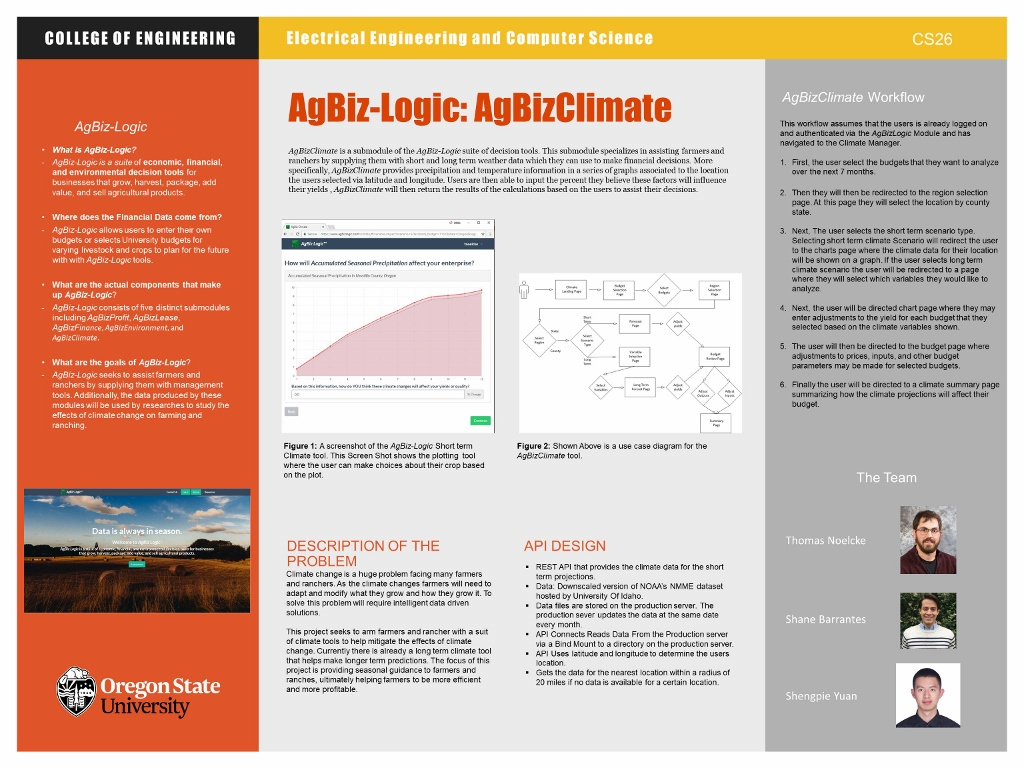
\includegraphics[width=22cm]{./Images/ExpoPosterGroup26.jpg}
    \end{landscape}
%We will put set up and configuration steps here. We will also discuss how our project works. Hardware and software requirements. User guids, API Docs.
% This section should cover:
% How does your project work?
%   What is its structure?
%   What is its theory of Operation?
%   Block flow and diagrams are good here.
%
% How does one install your software?
% How does one run your software?
% Are there any special run time requirements to run your software?
% Any user guides, API documentation etc.
%This needs to be detailed enough to recreate and/or use your project.
\section{Project Documentation}
    \subsection{Essential Documents}


    %This section will need to cover What websites were helpful?
    %What, if any, reference books really helped?
    %were there any people on campus that were really helpful?
    \subsection{Recommended Technical Resources}
        \subsubsection{Helpful web pages}

        \subsubsection{Helpful people on campus}
            \paragraph{Seam Hammond} Sean Hammond is our Clients technical adviser. When ever we ran into problems we weren't sure how to solve Sean was always our go to as he is very familiar with the project and the frame works used on the project.\\

            \paragraph{Rob Hess} Rob Hess is an instructor here on campus. He teaches web development, mobile development, cloud development and many other courses. During spring term Thomas and Shane were taking Rob's could development class where we were learning about vitalization. One of the problems we faced in this project was related to the best way to handle a vitalization problem at a design level. After coming up with a few ideas were able to run these by Rob and confirm that we were  using best practice for our problem.\\

            \paragraph{Graham Barber} Graham is a coworker of Thomas's at CASS here on campus. One day we were stuck on a docker compatibility issue with rocket and Graham was very helpful in helping us work through this issue. Graham has had some experience with rocket and was able to point us to some documentation that solved our problem.

            \paragraph{Zach Lerew} Zach Lerew is another one of Thomas's coworkers at CASS. Zach Lerew has had some experience with Django through work done at CASS. As a result when faced with some Django problems we were able to ask Zach for some help when facing issues that the documentation couldn't answer.\\

%This section should cover the following:
% What Technical information did you learn?
% What non-technical information did you learn?
% what have you learned about project work?
% what have learned about project management?
% what have you learned about working in teams?
% If you could do this all over again what would you do differently?

\section{Conclusions and Reflections}

    \subsection{Shane Barrantes}
        Over the course of this project I learned a lot about the following technologies.
        \begin{itemize}
            \item \textbf{Django:} I learned how the front-end, back-end, and unit tests work as well as how to add Routes and API Routes.
            \item \textbf{AngularJS:} I learned basic front-end information about angularJS and got a little bit of insight to how it's often tested.
            \item \textbf{Rkt:} I learned the limitations of pulling down containers and how to implement bind mounts.
            \item \textbf{NetCDF:} I learned what NetCDF, it's installation process, how to interact with files, and fairly deep understanding of the functionality.
            \item \textbf{Github:} I learned how to work in a team environment, how to squash merge conflicts, and how to re-base.
            \item \textbf{DevOps:} I learned about the deployment process for our project and gained some software building insights.
        \end{itemize}

        As far as non-technical information I learned how to frequently communicate with clients and how to work together in a team environment. I also learned how to work independently on a team project.

        I don't think I learned a whole lot about project work that I hadn't already experienced in a work or internship environment. One thing that stands out is time management while working with a team that has very different active hours than you do. Another thing I learned was how to regularly communicate the work progress directly to the client since.

        The project management skills I learned over the duration of this project mostly reside in inter-team communication and team scheduling. We frequently setup goals and deadlines that were in flux based on our term schedules, project state, and deadlines.

        The most important things I learned about working in teams are communication and of how to divide the work based on skills, availability, and fairness.

        If I could do this all over again I would look for an alternative solution for our client data API immediately. We took the client specification and tried our best to make it work, however this added months of work on tools and software that in the end were not used in the final product. If we were aware of our final solution sooner, we would have easily been able to do more testing and implement stretch goals.



    \subsection{Thomas Noelcke}



    \subsection{Shengpei Yuan}
			After finished project, I have learned several new skills.
			\begin{itemize}
					\item \textbf{Python:} I learned the difference between python 2.7 and 3, and used python to get data from climate website by modify parameter URL.
					\item \textbf{Django:} I learned unit tests, front-end and back-end.
					\item \textbf{NetCDF:} I learned how to install NetCDF and how it works with other files.
			\end{itemize}

			For the non-technical information, I have learned how to work and cooperate with teammate, and how to communicate with client when meet problem.
			After overviewed the project, I have learned the way using past climate data to predict the future yield of corps and understood the value of past climate data.
			For the project management, I have understood that plan ahead and finish task on schedule are very important because a complete project is the primary goal for the project management.
			For the team work, I have learned that communication is very important for the team and how to keep communication with group member.
			If I could do the project again, I would like to find more climate data sources and build a better data API to ensure project can get data anytime.


\section{Appendix}

    \subsection{Appendix 1: Essential Code Listings}

    \subsection{Appendix 2: Catch all}

\end{document}
